% This text is proprietary.
% It's a part of presentation made by myself.
% It may not used commercial.
% The noncommercial use such as private and study is free
% Sep. 2005 
% Author: Sascha Frank 
% University Freiburg 
% www.informatik.uni-freiburg.de/~frank/
%
% additional usepackage{beamerthemeshadow} is used
%  
%  \beamersetuncovermixins{\opaqueness<1>{25}}{\opaqueness<2->{15}}
%  with this the elements which were coming soon were only hinted
%\documentclass[8pt]{beamer}
\documentclass[10pt]{beamer}
\usepackage{etex}
\newenvironment<>{varblock}[2][\textwidth]{%
  \setlength{\textwidth}{#1}
  \begin{actionenv}#3%
    \def\insertblocktitle{#2}%
    \par%
    \usebeamertemplate{block begin}}
  {\par%
    \usebeamertemplate{block end}%
  \end{actionenv}}
%\usepackage{hyperref}
%\usepackage{natbib}
%\usepackage{beamerthemeshadow}
\usepackage{beamerinnerthemecircles, beamerouterthemeshadow}
\usepackage{marvosym}
\usepackage{amsmath,amssymb,amsfonts}
\usepackage[pdf]{pstricks}
%\usepackage{bbm}
%\usepackage{booktabs}
\usepackage{amsthm}
\usepackage{booktabs}
\usepackage{graphicx}
\usepackage{epsfig}
%\usepackage{graphics}

% MQ: This is to be able to compile on the Riksbank computer. Uncomment with my laptop. Ugly solution but will have to do for now.
%\usepackage{epstopdf}
%\epstopdfsetup{outdir=./}

\usepackage{rotating}

\usepackage{url}
\usepackage{breqn}
%\usepackage{hyperref}
\usepackage[authoryear]{natbib}
\usepackage{setspace}
\usepackage{multirow}
%\usepackage{harvard}
\usepackage{xcolor}
%\usepackage{multicolumn}
\usepackage{algpseudocode}
\usepackage{sidecap}
\usepackage{bbm} 
\usepackage{courier}
\usepackage{tikz}
\usetikzlibrary{arrows,shapes,snakes,automata,backgrounds,petri}

\tikzset{
  treenode/.style = {align=center, inner sep=0pt, text centered,
    font=\sffamily},
  arn_n/.style = {treenode, circle, white, font=\sffamily\bfseries, draw=black,
    fill=black, text width=1.5em},% arbre rouge noir, noeud noir
  arn_r/.style = {treenode, circle, red, draw=red, 
    text width=1.5em, very thick},% arbre rouge noir, noeud rouge
  arn_x/.style = {treenode, rectangle, draw=black,
    minimum width=0.5em, minimum height=0.5em}% arbre rouge noir, nil
}
\beamertemplatenavigationsymbolsempty

\newenvironment{myenumerate}{\begin{enumerate}[(1)]}{\end{enumerate}} 
\sidecaptionvpos{figure}{c}
% FOR COLORING PARTS  OF TABLE
%\usepackage[beamer,customcolors]{hf-tikz}

%\tikzset{hl/.style={
%    set fill color=red!80!black!40,
%    set border color=red!80!black,
%  },
%}

\mode<presentation> {
    \usetheme{Madrid} %Frankfurt} %Bergen, Berkely, Berlin, Boadilla, CambridgeUS, Darmstadt,
                          %Frankfurt, Goettingen, Singapore, Warsaw
    \usecolortheme{beaver} %seahorse} %default} %beetle, seahorse, wolverine, dolphin, beaver
    %\useoutertheme[subsection=true]{smoothbars} 
    \usefonttheme{default}
    %\usecolortheme{red}
    

	\setbeamercolor{block title}{use=unstructure, fg=white, bg=purple!75!black} %{use=structure,fg=white,bg=purple!75!black}
	%\setbeamercolor{block body}{use=structure,fg=black,bg=white!20!white}    
    %\setbeamercolor{block body}{bg=white}
    \setbeamertemplate{enumerate items}[default]
    \setbeamercolor{enumerate item}{fg=purple!75!black} 
    \setbeamercolor{enumerate subitem}{fg=purple!75!black} 	 
	\setbeamercolor{itemize item}{fg=purple!75!black}  
	\setbeamertemplate{itemize item}[triangle]  
	\setbeamercolor{itemize subitem}{fg=purple!75!black}
	\setbeamertemplate{itemize subitem}[triangle]
	\setbeamertemplate{blocks}[framed]


}



%\usepackage{colortbl}
%\definecolor{yellow}{cmyk}{0,0.18,0.90,0.00}

%\usepackage{xcolor}

%\usepackage[authoryear]{natbib}
\begin{document}
\title[Lecture 12]{Bayesian Learning 732A46: Lecture 12}  
\author[Matias Quiroz]{Matias Quiroz\inst{1}$^{,}$\inst{2}}
\setbeamerfont{institute}{size=\fontsize{7pt}{8pt}}
\institute[LiU and Riksbank]{
  \inst{1}%
   Division of Statistics and Machine Learning, Link\"{o}ping University\\~\\
  \inst{2}%
   Research Division, Sveriges Riksbank\\
     
}

%\institute[Riksbank and LiU]{Sveriges Riksbank and Division of Statistics and Machine Learning, Link\"{o}ping University}

\date[]{May 2016} %\today 

%\usebackgroundtemplate{%
%  \vbox to \paperheight{\vfil\hbox to \paperwidth{\hfil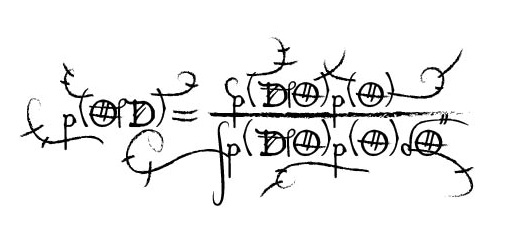
\includegraphics[width=1.5in]{Bayes.jpg}\hfil}\vfil}
%}

{
%\usebackgroundtemplate{\begin{center}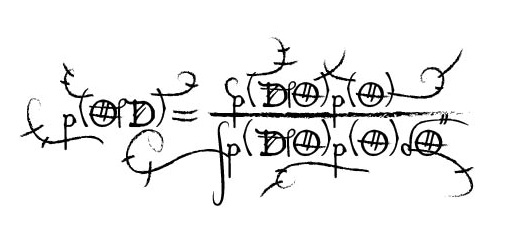
\includegraphics[width=0.4\paperwidth]{Bayes.jpg}\end{center}}
\usebackgroundtemplate{%
  \vbox to \paperheight{\hbox to \paperwidth{\hfil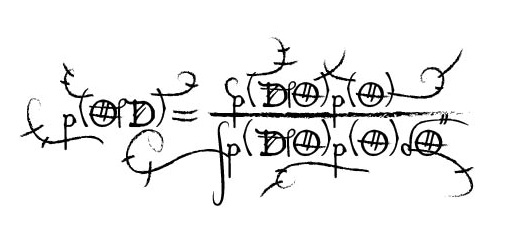
\includegraphics[width=2in]{Bayes.jpg}\hfil}}
}
\begin{frame}
\titlepage
\end{frame}
}
%\frame{\titlepage} 

%\frame{\frametitle{Overview of the talk}\tableofcontents}


\begin{frame}
\frametitle{Lecture overview}

\begin{itemize}
\item Hierarchical models
\bigskip
\item MCMC with RStan

\end{itemize}

\end{frame}



\begin{frame} %[fragile]
\frametitle{The normal Hierarchical model}
\begin{itemize}
\item \textbf{\color{blue}The  Bayesian hierarchical} normal model ($\mu$ and $\tau^2$ are also \textbf{\color{blue}random}!)
\begin{eqnarray*}
y_{ij} | \theta_j,\sigma^2 & \sim & \mathcal{N}(\theta_j, \sigma^2) \\
\theta_j | \mu, \tau^2 & \sim & \mathcal{N}(\mu, \tau^2) \quad \text{and}\quad \sigma^2 \sim p(\sigma^2) , \quad \mu, \tau^2 \sim p(\mu,\tau^2),
\end{eqnarray*}
where $i = 1, \dots, N$ (observations) and $j = 1, \dots, J$ (groups). Let $n_j$ be the \textbf{number of observations} in \textbf{group} $j$.
\item \textbf{\color{blue}Example}: $N=3$, $J=3$ and $\sigma^2$ known
\end{itemize}
\begin{center}
\begin{tikzpicture}[level 1/.style={sibling distance=3.5cm},
	level 2/.style={sibling distance=1cm}]


	\tikzstyle{state}=[circle,thick,fill=blue!20,minimum size=8mm]   
	\tikzstyle{empty}=[circle,draw=white!75,fill=white!20]  
	\begin{scope}
	\node[state]{$\mu,\tau^2$}
		child{ node [state]{$\theta_1$}
			child{ node [state]{$y_{11}$}}
			child{ node [state]{$y_{21}$}}
			child{ node [state]{$y_{31}$}} 	
		}
		child{ node [state]{$\theta_2$}
			child{ node [state]{$y_{12}$}}
			child{ node [state]{$y_{22}$}}
			child{ node [state]{$y_{32}$}}
		}
		child{ node [state]{$\theta_3$}
			child{ node [state]{$y_{13}$}}
			child{ node [state]{$y_{23}$}}
			child{ node [state]{$y_{33}$}}
		}	
		;
	\end{scope}

\end{tikzpicture}
\end{center}

\end{frame}



\begin{frame} %[fragile]
\frametitle{Some remarks on a hierarchical model}
\begin{itemize}
\item \textbf{\color{blue}Note}: the (unconditional/marginal) prior for $\theta$ is $$p(\theta)=p(\theta_1, \dots, \theta_J)= \int \left(\prod_{j=1}^N p(\theta_j|\mu, \tau^2)\right) p(\mu, \tau^2) d\mu d\tau^2.$$
\item $\theta_1, \dots, \theta_J$ \textbf{\color{red}are not} independent because
$$p(\theta_1, \theta_2, \dots, \theta_J) \neq p(\theta_1)p(\theta_2) \cdots p(\theta_J), \text{ but they are \textbf{\color{blue}exchangeable}.}$$
\item \textbf{\color{blue}Exchangeable}: $p(\theta)$ invariant to \textbf{permutation of indices}. \textbf{Weaker} than independence.
\item Hyper-parameters set to \textbf{\color{blue}sensible values} earlier. Modelling them now!
\vspace{-2mm}
\begin{center}
\begin{minipage}{\columnwidth}
\begin{varblock}[0.9\columnwidth]{\textbf{\color{yellow}Bayesian core philosophy}}
Regard unknown quantities as \textbf{\color{blue}random variables} and \textbf{\color{blue}learn from data}.
\end{varblock}
\end{minipage}
\end{center}\smallskip
\item Hierarchical models are \textbf{\color{blue}full probability models}... makes a Bayesian go {\Large{\Smiley}}\smallskip
\item \textbf{\color{blue}Practical advantages}? Shrinkage (=pooling in hierarchical terminology).
\end{itemize}
\end{frame}





\begin{frame}
\frametitle{The power of pooling (shrinking)}
\begin{center}
\begin{tikzpicture}[level 1/.style={sibling distance=3.5cm},
	level 2/.style={sibling distance=1cm}]


	\tikzstyle{state}=[circle,thick,fill=blue!20,minimum size=8mm]   
	\tikzstyle{empty}=[circle,draw=white!75,fill=white!20]  
	\begin{scope}
	\node[state]{$\mu,\tau^2$}
		child{ node [state]{$\theta_1$}
			child{ node [state]{$y_{11}$}}
			child{ node [state]{$y_{21}$}}
			child{ node [state]{$y_{31}$}} 	
		}
		child{ node [state]{$\theta_2$}
			child{ node [state]{$y_{12}$}}
			child{ node [state]{$y_{22}$}}
			child{ node [state]{$y_{32}$}}
		}
		child{ node [state]{$\theta_3$}
			child{ node [state]{$y_{13}$}}
			child{ node [state]{$y_{23}$}}
			child{ node [state]{$y_{33}$}}
		}	
		;
	\end{scope}

\end{tikzpicture}
\end{center}

\begin{itemize}
\item If $\tau^2\approx 0$ the ${\theta_j}$'s are close to each other ($\approx \mu$). The opposite for large $\tau^2$. \smallskip
\item To estimate the $\theta_j$'s {\color{red}the Frequentist} performs a \textbf{one-way ANOVA}. \smallskip
\item $H_0 = \textit{The means are equal {\color{blue}vs} } H_1 = \textit{The means are {\color{red}not} equal}. \text{ \textbf{F-test}.}$\smallskip
\item {\color{blue}$H_0$}: \textit{All data to estimate the common mean}. {\color{blue}$\neg H_0$}: \textit{Estimate each separately}. \smallskip
\item \textbf{\color{blue}Bayesian}: Why black or white? 
"To shrink completely or to not shrink at all" 
\end{itemize}

\end{frame}


\begin{frame}
\frametitle{The power of pooling (shrinking), cont.}
\begin{center}
\begin{tikzpicture}[level 1/.style={sibling distance=3.5cm},
	level 2/.style={sibling distance=1cm}]


	\tikzstyle{state}=[circle,thick,fill=blue!20,minimum size=8mm]   
	\tikzstyle{empty}=[circle,draw=white!75,fill=white!20]  
	\begin{scope}
	\node[state]{$\mu,\tau^2$}
		child{ node [state]{$\theta_1$}
			child{ node [state]{$y_{11}$}}
			child{ node [state]{$y_{21}$}}
			child{ node [state]{$y_{31}$}} 	
		}
		child{ node [state]{$\theta_2$}
			child{ node [state]{$y_{12}$}}
			child{ node [state]{$y_{22}$}}
			child{ node [state]{$y_{32}$}}
		}
		child{ node [state]{$\theta_3$}
			child{ node [state]{$y_{13}$}}
			child{ node [state]{$y_{23}$}}
			child{ node [state]{$y_{33}$}}
		}	
		;
	\end{scope}

\end{tikzpicture}
\end{center}

\begin{itemize}
\item \textbf{\color{blue}The Bayesian way:} \textbf{The data} decides the amount of pooling: $p(\tau^2|y)$.
\item {\color{blue}\textbf{\color{red}Extreme cases}} give the Frequentist solution
\begin{align*}
H_0 : \tau^2 & = 0 & \quad [\text{Shrink completely to }\mu] \\
H_1 : \tau^2 & = \infty & \quad [\text{Don't shrink at all}]
\end{align*}
\item Groups with \textbf{\color{red}few} $y_{ij}$'s: $H_1$ gives \textbf{\color{blue}high variance} on group mean estimates.
\item \textbf{\color{blue}Pooling to the rescue}: the estimates \textbf{borrow strength} from each other by \textbf{\color{blue}sharing hyper-parameters} (estimated using \textbf{all data} $y$)
\end{itemize}

\end{frame}

\begin{frame}
\frametitle{Estimation of the hierarchical normal model}
\begin{itemize}
\item \textbf{\color{blue}Blocks} of parameters: $\theta=\left\{(\theta_1, \dots, \theta_J), \sigma^2, \mu, \tau^2\right\}$.
\item The \textbf{\color{blue}joint posterior}
\begin{eqnarray*}
\pi(\theta) & \propto & p(y|\theta_1, \dots, \theta_J,\sigma^2, \mu,\tau^2)p(\theta_1, \dots, \theta_J, \sigma^2, \mu,\tau^2)\\
~ & = & p(y|\theta_1, \dots, \theta_J,\sigma^2)p(\theta_1, \dots, \theta_J| \sigma^2, \mu,\tau^2)p(\sigma^2, \mu,\tau^2) \\
~ & = & p(y|\theta_1, \dots, \theta_J,\sigma^2)p(\theta_1, \dots, \theta_J| \mu,\tau^2)p(\sigma^2, \mu,\tau^2) \\
~ & = & \left(\prod_{j=1}^J \prod_{i=1}^{n_j}  \mathcal{N}(y_{ij}|\theta_j, \sigma^2)\right) \left(\prod_{j=1}^J \mathcal{N}(\theta_{j}|\mu, \tau^2)\right)p(\sigma^2, \mu,\tau^2)
\end{eqnarray*}
is a \textbf{\color{red}nightmare}... \textbf{But} assuming $p(\sigma^2, \mu,\tau^2)=\underbrace{p(\sigma^2)}_{\text{Inv-}\chi^2} \underbrace{p(\mu)}_{\mathcal{N}} \underbrace{p(\tau^2)}_{\text{Inv-}\chi^2}$
\vspace{-5mm}
\begin{enumerate}
\item $\theta_j~|\mathrm{rest},y \sim \mathcal{N}$, $j = 1, \dots, J$
\item $\sigma^2|\mathrm{rest},y \sim \text{Inv-}\chi^2$
\item $\mu~|\mathrm{rest},y \sim \mathcal{N}$
\item $\tau^2|\mathrm{rest},y \sim \text{Inv-}\chi^2.$
\end{enumerate}
\item \textbf{\color{magenta}Gibbs sampling}! 
\end{itemize}

\end{frame}


\begin{frame}
\frametitle{More complex hierarchical models}
\begin{itemize}
\item We are ({\color{red}of course}) \textbf{not limited} to just 2 layers.
\begin{itemize}
\item \textbf{\color{blue}$L$-layers with params $\gamma_1, \dots \gamma_L$}:
 Just crank the \textbf{\color{blue}Bayesian machine}
$$p(\gamma_1, \dots, \gamma_L|y) \propto p(y|\gamma_1, \dots, \gamma_L)p(\gamma_1, \dots, \gamma_L)$$
and \textbf{\color{blue}factorize the prior} with the formula we have used more than 1000 times $$p(\gamma_1,\dots, \gamma_L)= p(\gamma_L|, \gamma_{L-1} \dots, \gamma_2, \gamma_1)p(\gamma_2|\gamma_1)p(\gamma_1).$$
\item Derive \textbf{\color{blue}full conditionals} $\gamma_l|\mathrm{rest},y$ by choosing (if possible) a \textbf{\color{blue}conjugate prior}.
\item \textbf{\color{blue}Estimation}: \textbf{\color{magenta}Gibbs sampling}. Is any $\gamma_l$ of unknown form? \textbf{Metropolis-Hastings} within Gibbs (Lecture 9)! 
\end{itemize}
\bigskip 
\item We are ({\color{red}of course}) \textbf{not limited} to normal distributions for \textbf{\color{blue}the data} $y$.
\begin{itemize}
\item We have \textbf{conjugate priors} for some other models... 
\item ... and if we don't: \textbf{M-H within Gibbs} saves us!
\end{itemize}

\end{itemize}

\end{frame}

\begin{frame}
\frametitle{More complex hierarchical models, cont.}
\begin{itemize}
\item Can easily \textbf{\color{blue}be generalized} to a regression setting. \medskip
\item Make $\gamma_l$ a function of specific covariates in the $l$th layer. \textbf{\color{blue}Example}: 
\vspace{-2mm}
$$\gamma_l = g_l(x'_l \beta_l)\quad [g_l(x'_l \beta_l)= x'_l \beta_l \text{ if linear regression}]$$ \\

\item \textbf{Estimate} $\beta_l$. If normal model: \textbf{\color{blue}Bayesian linear regression} updates. \medskip
\item \textbf{\color{blue}Example}: \textbf{Analyzing performance of students}.\\ \smallskip
\textbf{\color{blue}Hierarchies}: \textbf{students} within \textbf{classes} within \textbf{schools} within \textbf{states}.\\ \smallskip
\textbf{\color{blue}Data}: 10 tests ($y=$ score) for each student during a year. Possible $x$'s
\begin{itemize}
\item \textbf{\color{blue}Student}: Male/female, junior/senior, education of parents, etc.
\item \textbf{\color{blue}Class}: Years of experience of teacher, number of students in class, etc.
\item \textbf{\color{blue}School}: Private/public, measures on geographical level, e.g. crimes, unemployment, etc.
\item \textbf{\color{blue}State}: Welfare policies, e.g. investments in schools, social securities, etc. 
\end{itemize}
\medskip %\pause
\item We are ({\color{red}of course}) \textbf{not limited} to a univariate response. \\ \textbf{\color{blue}Example}: For student $i$, $y_i = (\text{math score, english score, history score})$
\end{itemize}

\end{frame}

\begin{frame}
\frametitle{Revisiting regularization in the Bayesian spline model}
\begin{figure}[H]
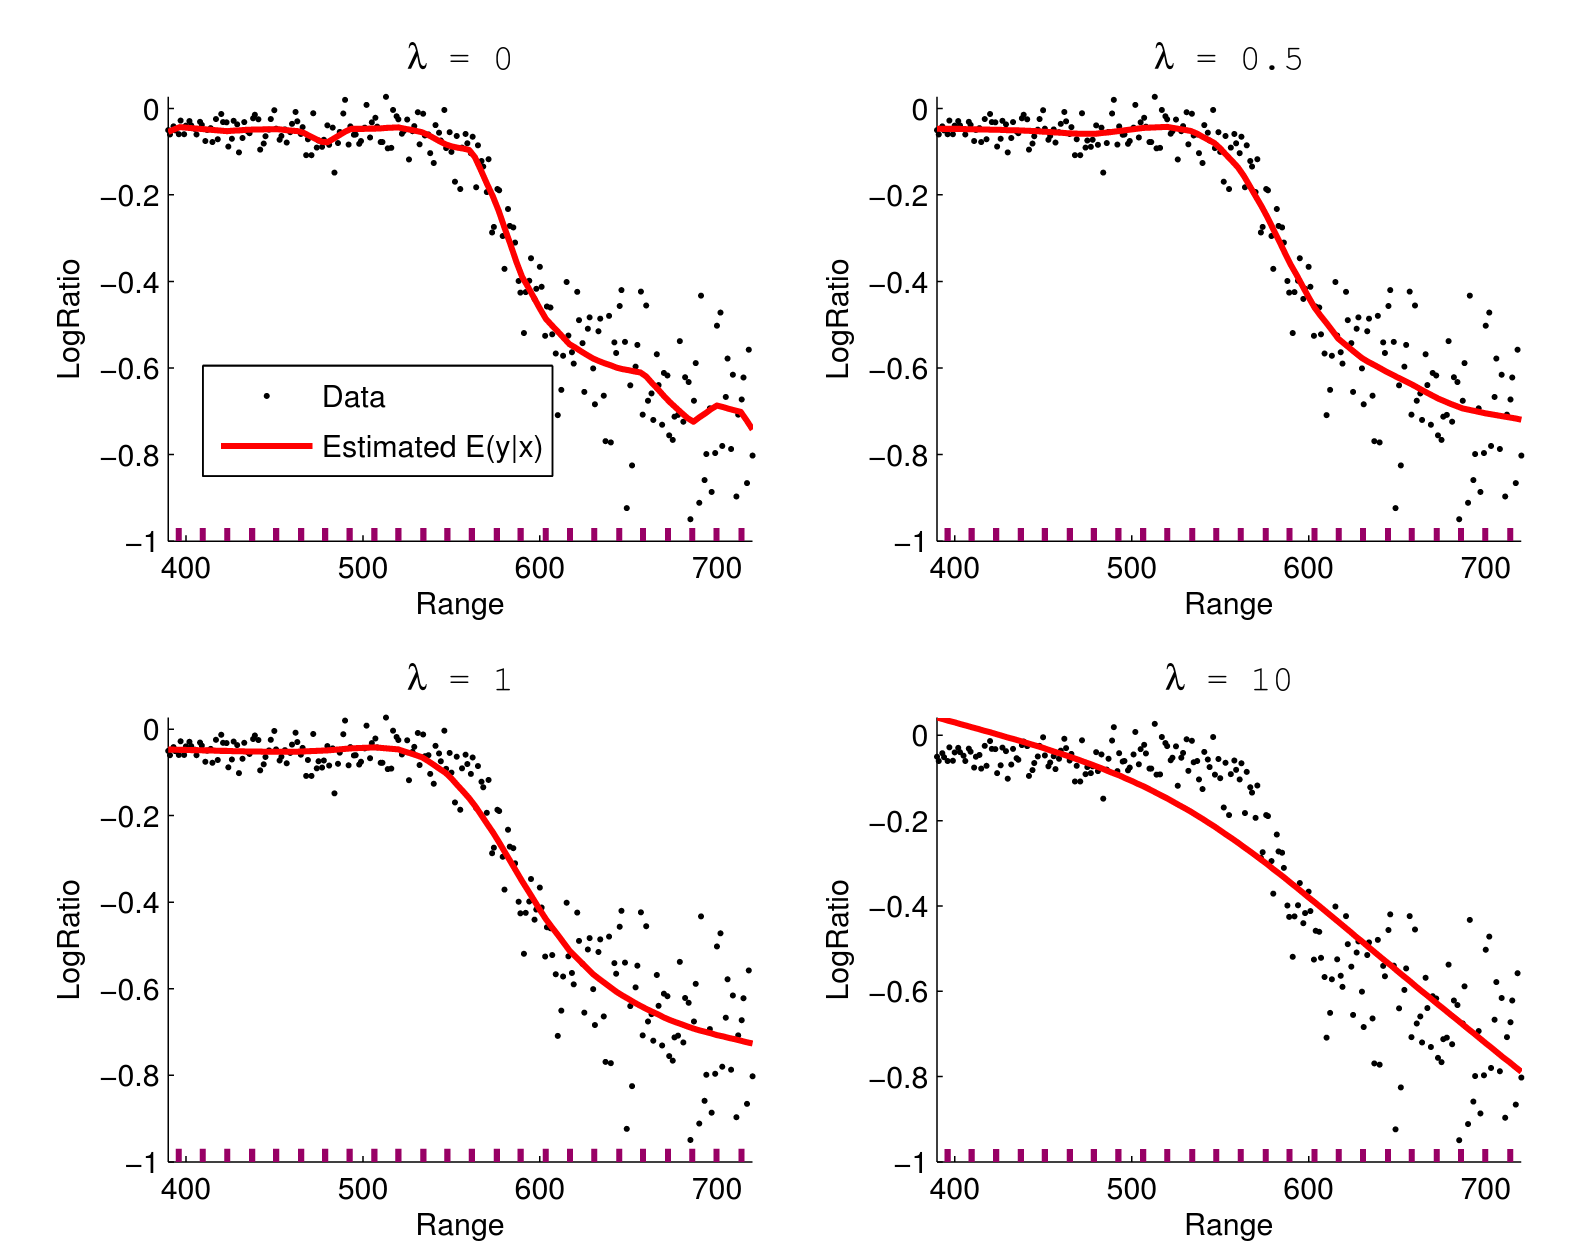
\includegraphics[width=0.8\columnwidth]{SplineFit}
%\protect\caption{LIDAR data.}
\end{figure}
\end{frame}


\begin{frame}
\frametitle{Estimating the shrinkage parameter $\lambda$ by direct sampling}
\begin{itemize}
\item \textbf{\color{blue}Model}: $y | \beta, \sigma^2 \sim \mathcal{N}(X\beta, \sigma^2 I)$
\item The \textbf{\color{blue}joint posterior} factorizes $$p(\beta,\sigma^2,\lambda|y) = p(\beta|\sigma^2,\lambda,y)p(\sigma^2|\lambda,y)p(\lambda|y),$$ where
\\~\\
\begin{tabular}{rcl}
$\textbf{\color{blue}Prior} \quad\quad\quad$ &  $\rightarrow$ & 
\vspace{3mm}
$\quad\quad\quad\textbf{\color{blue}Posterior}$ \\
\vspace{3mm}
$\beta | \sigma^2, \lambda \sim \mathcal{N}(0,\sigma^2\Omega_0^{-1})$ & $\rightarrow$ & $\beta|\sigma^2, \lambda, y \sim  \mathcal{N}(\beta_n, \sigma^2\Omega_n^{-1})$ \\
\vspace{2mm}
$\sigma^2 \sim \text{Inv-}\chi^2(\nu_0,s_0^2)$ & $\rightarrow$ & $\sigma^2 | \lambda, y \sim \text{Inv-}\chi^2(\nu_n,s_n^2)$ \\
$\lambda \sim p(\lambda)$ & $\rightarrow$ & $\lambda| y \sim  \sqrt{\frac{|\Omega_0 |}{|\Omega_n |}}\left(\frac{\nu_ns^2_n}{2}\right)^{-\nu_n/2} p(\lambda)$
%$p(\sigma^2)$ & $=$ & $\text{Inv-}\chi^2(\nu_0,s_0^2)$ & $\rightarrow$ & $p(\sigma^2|\lambda,y)$ & $=$ &$ \text{Inv-}\chi^2(\nu_n,s_n^2)$ \\~\\
%$p(\sigma^2)$ & $=$ & $\text{Inv-}\chi^2(\nu_0,s_0^2)$ & $\rightarrow$ & $p(\sigma^2|\lambda,y)$ & $=$ &$ \sqrt{\frac{|\Omega_0 |}{|\Omega_n |}}\left(\frac{\nu_ns^2_n}{2}\right)^{-\nu_n/2} p(\lambda)$
\end{tabular}
\\~\\ and \\~\\
\begin{tabular}{ll}
$\beta_n  =  (X^{\prime}X+\Omega_0)^{-1}X^{\prime}y  $ & $\Omega_n = X^{\prime}X+\Omega_0 $ \\
$\nu_n = \nu_0 + n $ & $\nu_n s^2_n = \nu_0s^2_0+y^{\prime}y - \beta_n^{\prime}\Omega_n \beta_n$
\end{tabular}
\item \textbf{\color{blue}Note}: $\beta$ and $\sigma^2$ dependent apriori to \textbf{achieve conjugacy}.
%$$p(\lambda|y) \propto \left(\frac{}{}\right $$
\end{itemize}
\end{frame}



\begin{frame}
\frametitle{Alternatively: make your life easy by a hierarchical setup}
\begin{itemize}
\item \textbf{\color{blue}Model}: 
\begin{align*}
y | \beta, \sigma^2  & \sim  \mathcal{N}(X\beta, \sigma^2 I)\\
\beta | \lambda  & \sim  \mathcal{N}(0, \Omega^{-1}_0) \quad \text{and } \sigma^2 \sim p(\sigma^2), \lambda \sim p(\lambda)
\end{align*}
and take (for example) $\Omega_0 = \lambda I$. \medskip
\item \textbf{\color{blue}Draw} the \textbf{hierarchical structure} (white board)! \medskip
\item Assuming $p(\sigma^2)=\text{Inv-}\chi^2$ and  $p(\lambda)=\text{Inv-}\chi^2$  [\textbf{\color{blue}semi-conjugate prior}] \textbf{•}
%\vspace{-5mm}
\begin{enumerate}
\item $\beta~| \mathrm{rest},y \sim \mathcal{N}$
\item $\sigma^2|\mathrm{rest},y \sim \text{Inv-}\chi^2$
\item $\lambda~|\mathrm{rest},y \sim \text{Inv-}\chi^2.$
\end{enumerate}\medskip
\item \textbf{\color{blue}That's easy}!... \medskip
\item ... \textbf{\color{red}But}: recall that Gibbs is \textbf{never as efficient} as \textbf{\color{blue}direct sampling}.

\end{itemize}

\end{frame}



\begin{frame}{RStan - a short demonstration}

\begin{itemize}
\item Why \textbf{\color{blue}Stan} (\href{http://mc-stan.org}{mc-stan.org})
\begin{itemize}
\item \textbf{Easy} to install (see \href{https://github.com/stan-dev/rstan/wiki/RStan-Getting-Started}{here}).
\item \textbf{Easy} to use.
\item \textbf{Efficient} MCMC. \textbf{\color{blue}Hamiltonian Monte Carlo}.
\item Integrates nice with \textbf{\color{blue}RStudio}.
\item Wrappers from \textbf{Python}, \textbf{R}, \textbf{Matlab}, \textbf{Stata}, \textbf{Julia}.
\item Good documentation.
\end{itemize}
\medskip
\item Alternatives to \textbf{Stan} (\textbf{Stan}islaw Ulam)
\begin{itemize}
\item Do it yourself \Smiley
\item \textbf{BUGS} (\textbf{B}ayesian inference \textbf{U}sing \textbf{G}ibbs \textbf{S}ampling)
\item \textbf{JAGS} (\textbf{J}ust \textbf{A}nother \textbf{G}ibbs \textbf{S}ampler)

\end{itemize}
\medskip
\item More examples found on the \textbf{\color{blue}course web page} and the \textbf{\color{blue}GitHub-repo}...
\medskip
\item ... and using your friend \textbf{\color{blue}Google}.
\end{itemize}
\end{frame}


\begin{frame}{The parts of a model in Stan}

\begin{itemize}
\item \textbf{\color{red}Six parts} in a \textbf{\color{blue}Stan} model:
\medskip
\begin{itemize}
\item \texttt{data}\medskip
\item \texttt{transformed data} \medskip
\item \texttt{parameters} \medskip
\item \texttt{transformed parameters} \medskip
\item \texttt{model} \medskip
\item \texttt{generated quantities} 
\end{itemize}
\end{itemize}
\end{frame}

\begin{frame}{Example: Poisson regression}

\begin{itemize}
\item \textbf{\color{blue}Poisson regression} for the \textbf{Number of roaches caught in buildings}.\smallskip
\item \textbf{\color{blue}Covariates}
\begin{itemize}
\item Exposure 
\item Treatment (yes/no)
\item Senior building (yes/no).
\end{itemize}\smallskip
\item \textbf{\color{red}Non-conjugate} model. \smallskip
\item \textbf{\color{blue}Model}:
\begin{align*}
y_i | \beta   & \sim \mathrm{Poisson}(\lambda_i)\\
\log( \lambda_i) & = \log(\mathrm{exposure}_i) +\beta_{1}+\beta_{2}\cdot\mathrm{treatment}_i+\beta_{3}\cdot\mathrm{senior}_i\\
\beta  & \sim \mathcal{N}(0, 1000) 
\end{align*} 


\end{itemize}
\end{frame}




\begin{frame}{Model in Stan: \texttt{data}}

\begin{itemize}
\item Read in \textbf{\color{blue}data} (done once)
\begin{itemize}
\item Variable declarations
\item A lot of different data types, e.g. \texttt{int}, \texttt{real}, \texttt{vector}, \texttt{matrix}.
\end{itemize}
\end{itemize}

\begin{center}
\begin{minipage}{\columnwidth}
\begin{varblock}[0.9\columnwidth]{\textbf{Example}: {\color{yellow}\textbf{\texttt{Data block}}}} 
\texttt{data \{}

\texttt{~~~int<lower=0> N; \# The number of observations}

\texttt{~~~int<lower=0> y; }

\texttt{~~~vector{[}N{]} exposure2; }

\texttt{~~~vector{[}N{]} senior; }

\texttt{~~~vector{[}N{]} treatment; }

\texttt{\}}
\end{varblock}
\end{minipage}
\end{center}

\end{frame}

\begin{frame}{Model in Stan: \texttt{transformed data}}

\begin{itemize}
\item \textbf{\color{blue}Variable declarations} and \textbf{\color{blue}statements} (done once)
\item See Chapter V in the documentation for all functions that can be used.
\end{itemize}

\begin{center}
\begin{minipage}{\columnwidth}
\begin{varblock}[0.9\columnwidth]{\textbf{Example}: {\color{yellow}\textbf{\texttt{Transformed data block}}}} 


\texttt{transformed data \{}

\texttt{~~~vector{[}N{]} log\_expo;}

\texttt{~~~log\_expo <- log(exposure2); }

\texttt{\}}
\end{varblock}
\end{minipage}
\end{center}
\end{frame}

\begin{frame}{Model in Stan: \texttt{parameters}}

\begin{itemize}
\item \textbf{\color{blue}Parameters} that should be sampled. 
\item \textbf{\color{blue}Parameter declarations} only.
\end{itemize}
\begin{center}
\begin{minipage}{\columnwidth}
\begin{varblock}[0.9\columnwidth]{\textbf{Example}: {\color{yellow}\textbf{\texttt{Parameters block}}}} 


\texttt{parameters \{}

\texttt{~~~vector{[}3{]} beta;}

\texttt{\}}
\end{varblock}
\end{minipage}
\end{center}
\end{frame}

\begin{frame}{Model in Stan: \texttt{transformed parameters}}

\begin{itemize}
\item \textbf{\color{red}Note}: Make sure that you know \textbf{which parametrization is used}. \textbf{\color{magenta}One of the best advices I can ever give you}.
\item \textbf{\color{blue}Parameter declarations} and \textbf{\color{blue}statements}.

\end{itemize}

\begin{center}
\begin{minipage}{\columnwidth}
\begin{varblock}[0.9\columnwidth]{\textbf{Example}: {\color{yellow}\textbf{\texttt{Transformed parameter block}}} [not our example]} 

\texttt{transformed parameters \{}

\texttt{~~~real<lower=0> sigma;}

\texttt{~~~sigma <- 1.0 / sqrt(tau);}

\texttt{\}}
\end{varblock}
\end{minipage}

\end{center}
\end{frame}

\begin{frame}{Model in Stan: \texttt{model}}

\begin{itemize}
\item Declare the \textbf{\color{blue}priors} and \textbf{\color{blue}model for data} with "sampling statement" symbol $\sim$.
\item \textbf{Distributions} can be found in Chapter VI and VII in the documentation.
\item \textbf{\color{red}Again}: Make sure that you know \textbf{which parametrization is used}.
\end{itemize}

\begin{center}
\begin{minipage}{\columnwidth}
\begin{varblock}[0.9\columnwidth]{\textbf{Example}: {\color{yellow}\textbf{\texttt{Model block}}}} 

\texttt{model \{}

\texttt{~~~\# Priors }

\texttt{~~~beta $\sim$ normal(0.0, 1000.0); }


\texttt{~~~\# Model }

\texttt{~~~y $\sim$ poisson\_log(log\_expo + beta{[}1{]}
+ \\ ~~~beta{[}2{]} {*} treatment + beta{[}3{]}{*}senior);}

\texttt{\}}
\end{varblock}
\end{minipage}
\end{center}
\end{frame}

\begin{frame}{Model in Stan: \texttt{generated quantities}}

\begin{itemize}
\item Post sampling computations. \textbf{\color{blue}Examples}:
\begin{itemize}
\item Model checking
\item Posterior predictive distribution
\item Applying full Bayesian decision theory
\item Transforming parameters for reporting.
\end{itemize}
\end{itemize}

\begin{center}
\begin{minipage}{\columnwidth}
\begin{varblock}[1\columnwidth]{\textbf{Example}: {\color{yellow}\textbf{\texttt{Generated quantities block}}}} 

\texttt{generated quantities \{}

\texttt{~~~int<lower=0> pred_treat; }

\texttt{~~~int<lower=0> pred_notreat; }

\texttt{~~~vector[3] exp_beta;}

~\\
\texttt{~~~exp_beta <- exp(beta);}

\texttt{~~~pred_treat <- poisson_rng(exp_beta[1]*exp_beta[2]);}

\texttt{~~~pred_notreat <- poisson_rng(exp_beta[1]);}

%  exp_beta <- exp(beta);
%  pred_treat <- poisson_rng(exp_beta[1]*exp_beta[2]);
%  pred_notreat <- poisson_rng(exp_beta[1]);


%  int<lower=0> pred_notreat;
%  vector[3] exp_beta; 
%
%  exp_beta <- exp(beta);
%  pred_treat <- poisson_rng(exp_beta[1]*exp_beta[2]);
%  pred_notreat <- poisson_rng(exp_beta[1]);


%\texttt{~~~my\_weight\_pred <- alpha + beta {*} MySHeight + normal\_rng(0,sigma); }

\texttt{\}}

\end{varblock}
\end{minipage}
\end{center}

%\begin{center}
%\begin{minipage}{\columnwidth}
%\begin{varblock}[0.9\columnwidth]{\textbf{Example}: {\color{yellow}\textbf{\texttt{Generated quantities block}}}(not example model)} 

%\texttt{generated quantities \{}

%\texttt{~~~real my\_weight\_pred; }

%\texttt{~~~my\_weight\_pred <- alpha + beta {*} MySHeight + normal\_rng(0,sigma); }

%\texttt{\}}

%\end{varblock}
%\end{minipage}
%\end{center}
\end{frame}

%# BEGIN PASTE
%  int<lower=0> pred_treat;
%  int<lower=0> pred_notreat;
%  vector[3] exp_beta; 
%
%  exp_beta <- exp(beta);
%  pred_treat <- poisson_rng(exp_beta[1]*exp_beta[2]);
%  pred_notreat <- poisson_rng(exp_beta[1]);
%
%# END PASTE


\begin{frame}{Demonstration}
\begin{center}
\Large{\texttt{Demonstration on my computer}}
%\Large{\texttt{Demonstration}}
\par\end{center}
\end{frame}

\begin{frame}
\frametitle{This is the End...}
\begin{figure}[H]

\includegraphics[width=0.40\columnwidth]{PayesBayes}
%\protect\caption{The good$\p(\alpha, \beta|y)$}
\end{figure}


\begin{itemize}
\item .. \textbf{\color{blue}of my lectures}..
\item ... \textbf{but the Beginning} of \Large{\textbf{\color{blue}your new life as a Bayesian}}.
\item \textbf{\color{magenta}Thank you}, it has been a pleasure.
\end{itemize}
\end{frame}



\end{document}

